\chapter{Introduction\label{ch:intro}}

The utilization of combustion has been a crucial part of civilization.  From an engineering point of view, the efficiency, reliablity, and emissions of combustion processes are still to be further improved.  The combustion processes in a gas turbine engine, for example, involve fuel and air mixing, stabilization of the flame, and emissions of imcomplete combustion products and nitrogen oxides.  From a fundamental research point of view, understanding and optimizing each of these processes to achieve high-efficiency low-emission combustion is not trivial.  This is due to the fact that combustion is interdisciplinary: it is a scientific discipline that studies the coupling between chemical kinetics and fluid dynamics, both of which are challenging by themselves.  

On chemical kinetics, due to the large number of intermediate species and elementary reactions during the thermal pyrolysis and oxidation of fuels, the development and validations of chemical models are very challenging.  As shown in the Lu-Law diagram~\cite{lu09}, the size of the chemical model grows significantly with increasing size of fuel molecules.  To date, some large chemical models contain as many as a few thousand species and tens of thousand reactions~\cite{lu09}.  

On fluid dynamics, complexities lie in turbulence, multi-time and multi-length scale transport, and the nonlinear nature of the Navier-Stokes equations.  Especially in turbulent reacting flows, temporally and spatially well resolved measurements are only available for certain quantities, while detailed numerical simulations that can capture the unsteadiness and fine structures in the flow field can be computationally intensive due to the broad range of length/time scales that requires many orders of magnitude in resolution.

However, as already mentioned, in practical combustion systems, where realistic fuel mixtures react in turbulent flows, chemical kinetics and fluid dynamics are strongly coupled, which brings in further complexities.  Therefore, simplifications of chemistry or flow are often made to reduce ambiguities in such systems to unravel the coupling effects.  For example, the role of chemical kinetics are often studied in homogeneous systems, where transport is negligible.  Conversely, in turbulent combustion studies, simple fuels are often used to minimize the uncertainty in chemistry.  

The overall objective of this dissertation is to elucidate the chemistry-transport couplings in combustion and emission at practical engine relevant conditions.  Specifically, flame dynamics (ignition/extinction/stabilization) and soot emissions are invesigated.  For both topics, the complexity of the coupling effect is gradually increased by first studying detailed chemical kinetics in one-dimensional laminar flows and then advancing to multi-dimensional (turbulent) configurations.  

\section{Chemistry-Transport Coupling in Flame Dynamics}

The first half of this dissertation focuses on the coupling effects of chemical kinetics and transport in flame dynamics.  An overarching issue here is the potential role of low-temperature chemistry in constituting a flame structure, the interaction of such a low-temperature flame with flow, and their relevance in practical engine combustion.  To approach this question, a general overview on low-temperature chemistry and resulting cool flames is presented first.  Evidence showing that low-temperature chemistry can be important for flame dynamics (ignition/extinction/stabilization) are then provided to further motivate this part of work.

\subsection{Low-Temperature Chemistry and Cool Flames}\label{sec:intro-NTC-generic}

Cool flames, first reported in 1817~\cite{davy17}, are controlled by low-temperature chemical kinetics that have been extensively studied ever since~\cite{griffiths87}.  Such low-temperature chemistry (LTC) is ubiquitous for most hydrocarbon fuels and has been shown to be closely related to the negative temperature coefficient (NTC) phenomenon observed in autoignition processes~\cite{ciezki93,hwang08} and engine knock~\cite{griffiths02}.  Practical hydrocarbon-based fuels generally have two-stage ignition processes, in which the first stage ignition is governed by low-temperature chemistry and the second stage ignition by high-temperature chemistry.  In both low- and high-temperature regimes, the ignition delay time decreases as the initial temperature increases.  However, in the intermediate-temperature regime, the transition of the ignition chemistry results in increased overall ignition delay time as the initial temperature increases.  Negative temperature coefficient refers to the phenomenon that the ignition delay time of a fuel/air mixture increases with increasing initial temperature within a certain low-to-intermediate temperature range in relation to its adiabatic flame temperature.  This range is typically between $600$ and $800$ K at $1$ atm, which is relatively low compared to a typical flame temperature of 2000 K.  Therefore, the terminologies of low-temperature chemistry, NTC chemistry, and cool flame chemistry are often used interchangeably.  

The fundamental understanding of low-temperature chemistry and cool flame dynamics can be important for combustion phasing control in the recent development of homogeneous charge compression ignition (HCCI) engines~\cite{lu11} and reactivity controlled compression ignition (RCCI) engines~\cite{kokjohn11}.  For example, cool flames and NTC phenomena have been mostly observed in homogeneous systems such as rapid compression machines~\cite{silke05,mittal08,di14}, shock tubes~\cite{ciezki93,herzler05,vasu08}, flow reactors\cite{koert94,curran00} and stirred reactors~\cite{dagaut95,veloo13,kikui15}.  Without the complexity of inhomogeneity and transport, low-temperature chemical kinetics can be studied in these systems for chemical model development.  However, in practical combustors such as diesel and gasoline direct injection (GDI) engines, combustion processes are governed by both transport and chemical kinetics.  At such conditions, the characteristic mixing time scales are comparable to the chemical reaction time scales, and the convective-diffusive processes may affect the initiation and development of cool flames.  It is reasonable to expect that, in chemically reacting flow, when the characteristic transport time becomes comparable to the NTC chemical time, the two processes will be strongly coupled to affect the local response.  By the same reasoning, when the characteristic mixing time becomes relatively long, NTC chemistry will be decoupled from the transport processes, and the system response will recover to that of the homogeneous mixture.

\subsection{LTC in Nonpremixed Flames}\label{sec:intro-NTC-nonpremixed}

\begin{figure}[t]
  \centering
  \scriptsize
  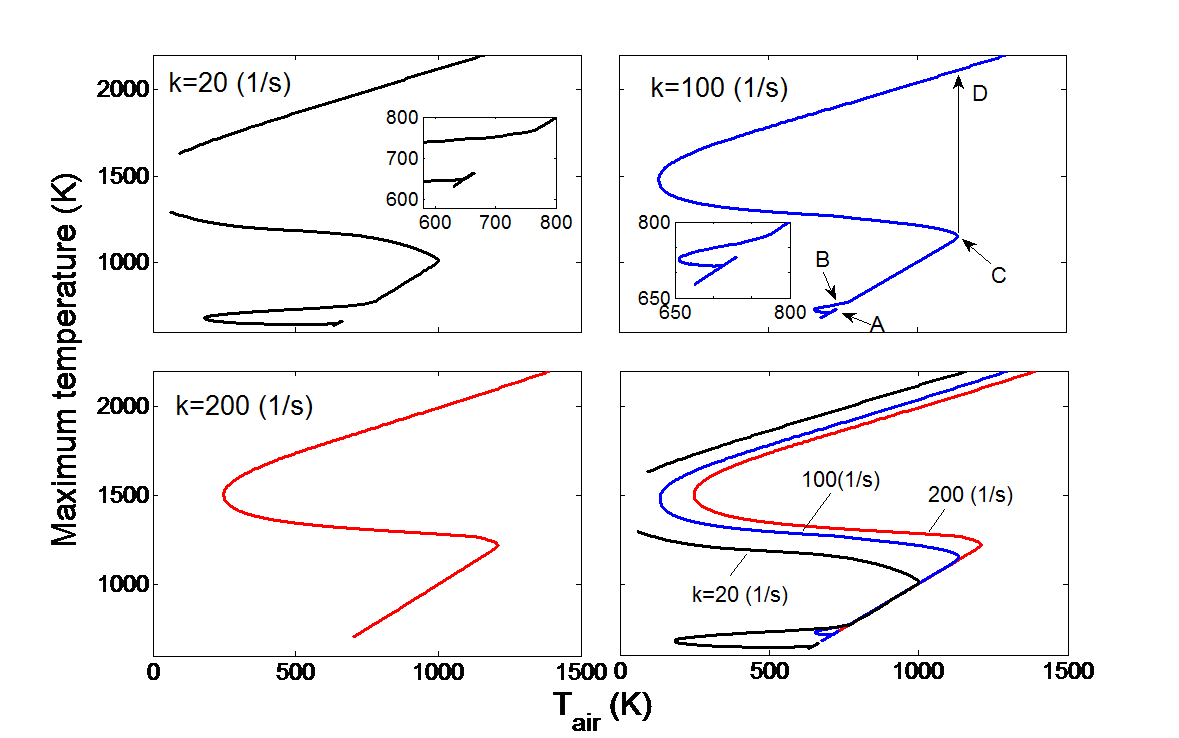
\includegraphics[width=1.0\textwidth]{ch-intro/scurve-zhao.png}
  \normalsize
  \caption{Figure 8 in Law and Zhao~\cite{law12}.  The global response S-curve plotted as maximum temperature versus air-side boundary temperature.  The strain rate varies from 20 to 100 to 200 /s, and the pressure is 1 atm.}
  \label{fig:scurve-zhao}
\end{figure}

Cool flames in nonpremixed systems have been recently studied in counterflow flames~\cite{law12,zhao13,won15,ju16} and microgravity droplet combustion~\cite{nayagam12,farouk15,nayagam15}.  Specifically, Law and Zhao~\cite{law12} and Zhao and Law~\cite{zhao13} computationally investigated nonpremixed counterflow cool flames of $n$-heptane and identified the existence of a secondary S-curve dominated by low-temperature chemistry at low strain rates or high pressures, as shown in Fig.~\ref{fig:scurve-zhao}.  The steady-state response of a one-dimensional reactive system subjected to heat loss can be studied via the S-curve analysis~\cite{lawbook}.  In such an analysis, a system response such as the maximum temperature or radical concentration is monitored for variations of an imposed parameter such as the air temperature, for a given strain rate of the flow, or the system Damk\"ohler number.  For a global one-step overall reaction with large activation energy, the intrinsically nonlinear Arrhenius kinetics frequently yields multiple solutions characterized by an S-shaped response curve, with the lower and upper turning points respectively designate the ignition and extinction states of the system.  Such triple-branch S-curves also frequently emerge for simulations using detailed reaction mechanisms, while more complex response curves with additional turning points have also been obtained, for example for hydrogen oxidation~\cite{kreutz94,fotache98} and methane oxidation~\cite{liu09}.  However, as shown in Fig.~\ref{fig:scurve-zhao}, the secondary S-curve, computationally obtained by Law and Zhao, has its own ignition and extinction turning points and grafts on the lower branch of the primary S-curve. This secondary S-curve predicts the existence of  nonpremixed cool flames at certain conditions.    

Moreover, in microgravity droplet combustion, it was found that the visible flame of large $n$-heptane, $n$-octane, and $n$-decane droplets could transit to a quasi-steady low-temperature-burning mode after extinction of the hot flame due to radiation, suggesting the existence of steady droplet burning sustained by a cool flame~\cite{nayagam15}.   

In Chapter~\ref{ch:NTC} of the dissertation, the computationally predicted nonpremixed counterflow cool flames were experimentally explored.  Ignition and extinction states of nonpremixed cool flames were quantified to provide validation data for further development of low-temperature chemical models.  Computations with detailed chemistry and transport were then conducted to elucidate the thermal and chemical structure of the nonpremixed cool flames, which lays the foundation for understanding the coupling effects of low-temperature chemistry and transport in more complex flows and flame stabilization.

\subsection{Nonpremixed Flame Stabilization and Oscillation}\label{sec:intro-stabilization}

\begin{figure}[t]
  \centering
  \scriptsize
  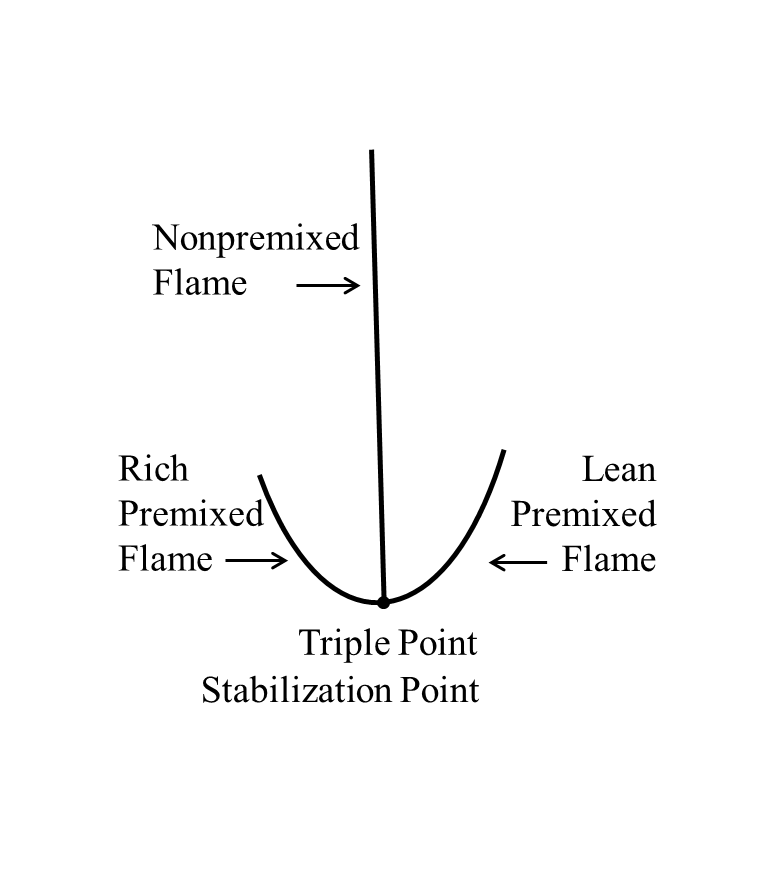
\includegraphics[trim=20mm 24mm 20mm 20mm, clip=true, width=0.5\textwidth]{ch-intro/triple_flame.png}
  \normalsize
  \caption{A schematic plot of the tribrachial flame structure in a coflow mixing layer.}
  \label{fig:triple_flame}
\end{figure}

Nonpremixed jet flames have been extensively studied to understand combustion processes in rocket and diesel engines.  The stabilization and structure of jet flames determine the lift-off height of the flame and are therefore integral to engine design.  Due to the mixing process of the fuel and oxidizer streams in lifted flames at nonautoignitive conditions, the combustion mode is partially premixed, leading to the observation of a two-dimensional tribrachial flame (also known as triple flame)~\cite{buckmaster02}; specifically, a lean and a rich premixed flame wings with a trailing diffusion flame branch, as shown in the schematic plot in Fig.~\ref{fig:triple_flame}.  The point where the three branches intersect is called the triple point and is generally considered to be the stabilization point for nonautoignitive situations. The dynamic balance between the local flame propagation speed and the incoming flow speed is characterized as the stabilization mechanism.  A recent review by Chung~\cite{chung07} discussed the stabilization, propagation, and instability of tribrachial flames, including the effects of concentration gradient~\cite{dold89,hartley91,ghosal00}, velocity gradient~\cite{kim07}, and burned gas expansion~\cite{ruetsch95,lee97,plessing98,kioni99}.  These studies, however, were limited to nonautoignitive conditions, while real engines operate at elevated pressures and temperatures, where autoignition is activated and could interact with the tribrachial flame.

Chung and co-workers~\cite{choi09,choi10,choi12} further conducted a series of experiments to investigate the autoignition characteristics of laminar C$_1$ to C$_4$ fuel jets in a heated air coflow and found that, above certain coflow temperatures, lifted flames could be established through autoignition.  In these studies, both the tribrachial structure for most autoignited cases and a repetitive behavior of extinction and reignition at the critical condition near blowout were observed.  It has been found that the ignition delay time plays an important role for the stabilization of autoignited lifted flames, in such a way that the autoignited liftoff height was correlated with the square of the ignition delay time in some of the investigated cases.

Besides the elevated temperature and pressure effects that initiate autoignition, unsteady flow motion can also modify the flame structure in nonpremixed coflows.  For example, in the experimental investigation of Strawa and Cantwell~\cite{strawa89}, flow instability and flame breakup was achieved by imposing a small-amplitude, periodic velocity fluctuation to nonpremixed jet flames at elevated pressures and low Reynolds numbers.  Later, in the computational study of S\'{a}nchez-Sanz~\emph{et al.}~\cite{sanchezsanz10}, perturbation frequency effects on the thermal and chemical properties of the flame in such periodically time-varying flows were evaluated.  Three regimes were found depending on the flame's Strouhal number, $S = Df/2U$, with $D$ and $f$ denoting the fuel jet diameter and perturbation frequency, respectively.  For small Strouhal numbers ($S = 0.1$), perturbations can travel far downstream, resulting in an oscillating flame.  Flame surface flickering was observed when $S\simeq 0.2$, and vigorous flame pinch-off was observed at $S = 0.5$.  Larger values of $S$ confine the oscillation to the jet's near-exit region with the pulsation having minimal effects on temperature and concentration values.  The unsteadiness in flickering flames also increases pollutant formation, such as soot~\cite{shaddix94} and carbon monoxide~\cite{skaggs96}.  Mohammed~\emph{et al.}~\cite{mohammed98} followed by Dworkin~\emph{et al.}~\cite{dworkin07} conducted computational and experimental studies of $20$ Hz periodically-forced methane/air coflow diffusion flames.  Acetylene production increased~\cite{mohammed98} and the oxidation of CO to CO$_2$ was inhibited~\cite{dworkin07} in the downstream region of the flame at certain times during the flame's cyclic history. 

\subsection{LTC in Flame Stabilization}\label{sec:intro-NTC-stabilization}

As reviewed in previous sections, low-temperature chemistry can induce two-stage ignition and is promoted at elevated pressures.  Consequently, NTC-affected stabilization of nonpremixed lifted jet flames can be potentially important, yet few studies have performed any detailed analysis.  Krisman \emph{et al.}~\cite{krisman15} recently conducted a numerical study of dimethyl ether (DME)/air mixing layer at $40$ atmospheres and air coflow temperatures ranging from $700$ to $1500$ K and observed multibrachial structures in the heat release rate profiles.  The mixture fractions (local composition states) corresponding to the stabilization points defined based on the hydroxyl radical (OH) mass fraction, and the first stage autoignition kernels based on the methoxymethylperoxy radical (CH$_3$OCH$_2$O$_2$), were compared with the most reactive mixture fractions computed from homogeneous autoignition under the same initial conditions.  A transport budget analysis based on selected species was performed to differentiate deflagration from autoignition.

In light of the reported multibrachial structure, showing a modified flame shape from autoignition in the mixing layer, further investigation is warranted to identify the detailed chemical structure and stabilization mechanism of the multibrachial flame.  For example, tools for computational diagnostics, especially for identifying locally dominant chemical reactions, can be employed to understand the controlling chemistry.  Moreover, a direct comparison to homogeneous autoignition is insufficient to understand the transport processes in the current configuration.  In the two-dimensional mixing layer, transport processes in two directions are important: parallel and normal to the mixture fraction gradient, which are due to the transverse stratification of temperature and species and streamwise flow and (flame back) diffusion, respectively.  These considerations would significantly improve the understanding of the role of autoignition upstream of the flame structure and quantitatively identify the controlling kinetics and stabilization mechanism.

In Chapter~\ref{ch:dynamics} of this dissertation, nonpremixed coflow flame dynamics under autoignitive conditions were computationally investigated.  Leveraging the understanding of low-temperature chemistry obtained from nonpremixed counterflow cool flame studies in Chapter~\ref{ch:NTC}, the role of NTC chemistry in flame stabilization at engine relevant conditions will be elucidated.  Moreover, the dominant stabilization mechanism at various flow conditions and the effect of unsteadiness on flame dynamics will be investigated to demonstrate the coupling of fluid dynamics and chemical kinetics to further facilitate future turbulent studies.

\section{Chemistry-Transport Coupling in Soot Emissions}

The second half of this dissertation focuses on the coupling effects of chemical kinetics and transport in sooting flames.  A general question that governs the subsequent investigations is how soot evolution happens in practical engine combustion.  To approach this question, a general overview on soot formation and emission is presented first.  Fuel and flow effects on soot evolution are then reviewed to further motivate this part of work.

\subsection{Soot Mechanisms and Emissions}\label{sec:intro-soot-generic}

In addition to flame dynamics, emissions from combustion processes are also subject to the coupling effects of chemical kinetics and flow dynamics.  One of the dominant pollutants that appears in the form of particulate matter (PM) is carbon black or soot.  Soot particles are undesired products of rich combustion in a wide variety of engineering and natural systems, including transportation and propulsion engines, power generation devices, and fires.  Significant exposure to these black nanoparticles is known to cause heart diseases or lung cancer~\cite{donaldson05}.  In addition, particles emitted from aircraft engines enhance nucleation in the formation of contrails and other atmospheric aerosols~\cite{jensen97,seinfeldbook98}.  Because of the adverse effects on human health and the environment, stringent regulations on emissions from automotive and aircraft engines have been proposed by governments worldwide.

\begin{figure}[t]
  \centering
  \scriptsize
  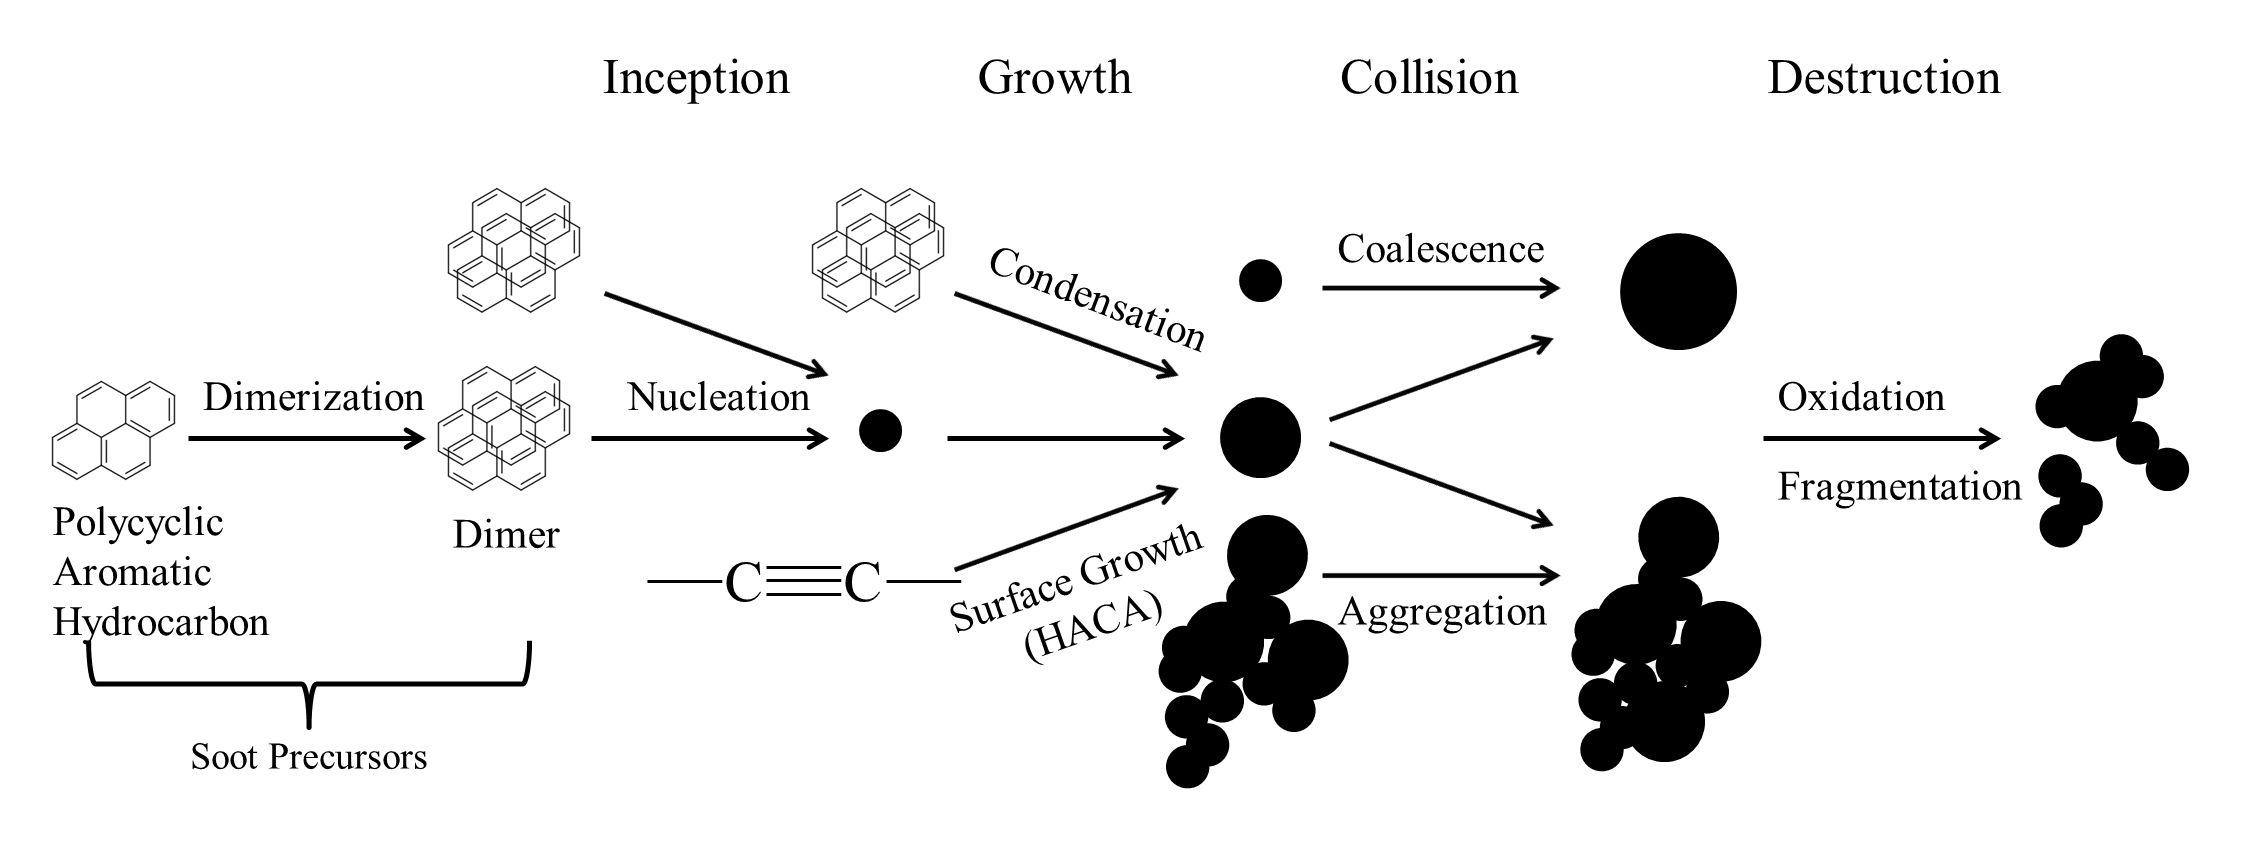
\includegraphics[width=1.0\textwidth]{ch-intro/soot.png}
  \normalsize
  \caption{A schematic drawing of the physical and chemical processes that govern soot evolution.}
  \label{fig:soot}
\end{figure}

The evolution of soot particles is governed by both physical and chemical processes, and the exact mechanisms of soot evolution remain open questions in varying degrees.  A general soot model includes inception, growth, collision, and destruction of soot particles, as shown in the schematic drawing in Fig.~\ref{fig:soot}.  During the inception process, gaseous soot precursors nucleate to form the first soot particle~\cite{schuetz02,wong09,blanquart09c}.  Most soot models consider that these precursors originate in benzene and grow by addition of carbon atoms following the H-abstraction C$_2$H$_2$-addition (HACA) mechanism~\cite{frenklach91}.  Large hydrocarbon molecules are formed from the continuing growth of carbon atoms and appear in ring structures, generally referred as polycyclic aromatic hydrocarbons (PAH)~\cite{schuetz02}.  The subsequent soot growth processes are also closely related to PAH and acetylene, through physical condensation~\cite{park03,mitchell98,mitchell03} and chemical surface growth with the HACA mechanism~\cite{frenklach91}, respectively.  The collision between soot particles also modifies soot morphology.  Two extreme cases are demonstrated in Fig.~\ref{fig:soot}: two small soot particles completely merge to a big spherical particle, or they just barely stick to each other, preserving the total surface area.  Experimentally, soot particles have been found to be both spheres~\cite{zhao05} and fractal aggregates~\cite{jensen07}, as shown in Fig.~\ref{fig:TEM}.  Finally, if the soot particles are exposed to oxidizers such as oxygen and hydroxyl radical, soot fragmentation and oxidation may occur~\cite{kazakov95,neoh81}, resulting in the destruction of soot particles.

\begin{figure}[t]
  \centering
  \scriptsize
  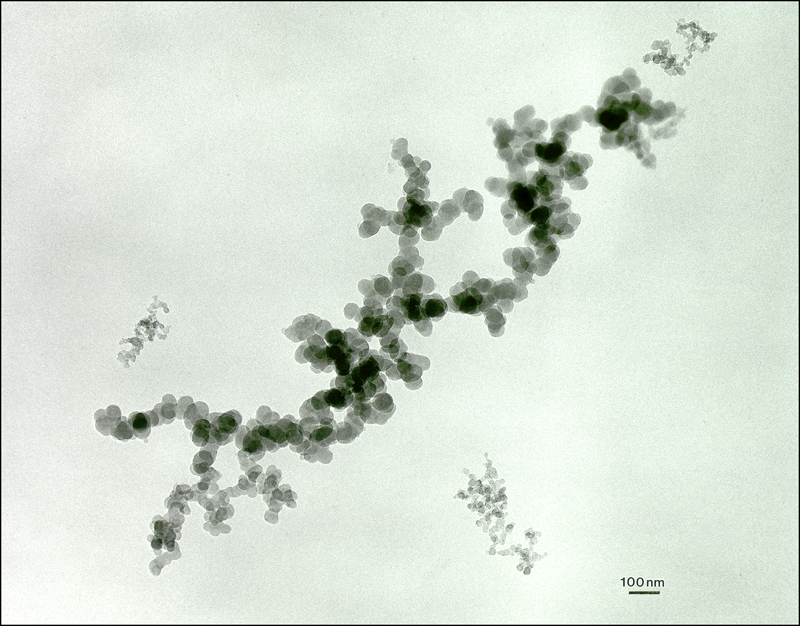
\includegraphics[width=0.6\textwidth]{ch-intro/TEM.jpg}
  \normalsize
  \caption{Transmission electron microscopy (TEM) images of soot aggregate from Jensen \emph{et al.}~\cite{jensen07}.}
  \label{fig:TEM}
\end{figure}

Understanding of soot mechanism has been acquired through experiment and modeling.  While experiments provide data to guide model development and validation, modeling provides insights to help design experiments, improve experimental techniques and understand some of the mechanisms inaccessible in experiments.  However, large uncertainties are still associated with soot models in both the gas phase PAH chemistry and soot dynamics.  Due to limited optical access in sooting flames for online species measurement, validation data for PAH chemical model development is limited.  Therefore, how these large PAH species are formed from smaller species during the fuel breakdown processes needs to be investigated in well-controlled laminar experiments to obtain fundamental understanding of PAH chemical kinetics.  This will then allow the development of relatively high-fidelity soot models to be utilized in, for example, turbulent sooting flame computations to investigate soot evolution in practical engines, for detailed characterization of the flow field and soot would not be available due to experimental limitations.

\subsection{Role of Fuel Structure in PAH Chemistry and Soot Emissions}\label{sec:intro-biofuel}

The utilization of biofuels, which are potential partial replacements for liquid fuels derived from fossil fuels, is garnering wide attention not only because these fuels are renewable, locally producible, and carbon neutral~\cite{liu11} but they also hold potential for positive impacts on particulate matter emission control. Biofuels, including bioalcohols and biodiesels, mainly consist of oxygenated hydrocarbons, such as ethers, alcohols, and esters. When used as additives in conventional diesel fuels, PM emissions have been found to decrease as oxygenated additive concentrations increase~\cite{graboski98}.

However, the precise role of oxygenated additives on the reduction of soot emission has not yet come to a scientific consensus. For example, Frijters and Baert~\cite{frijters06} attributed the PM reduction to the fuel oxygen content, which reduced the local equivalence ratio and, by implication, the flame temperature.  However, even with the same oxygen content, the oxygenates have different efficiencies in the reduction of soot precursor, as Westbrook \emph{et al.}~\cite{westbrook06} found through simulations of premixed $n$-heptane and oxygenates flames.  Furthermore, Pepiot \emph{et al.}~\cite{pepiot08} proposed a structural group contribution approach to interpret diesel engine experimental data and quantify the soot reduction tendency of oxygenated fuels.  As noted by the authors, the aromatics contained in the conventional diesel fuels have very strong sooting tendencies, which are moderated through substitution by the clean-burning oxygenated additives; this replacement effect should be identified and quantified to reveal the role of the oxygen moieties. 

Conversely, a number of studies show that oxygenated fuels do not necessarily have lower sooting tendencies than regular hydrocarbons.  McEnally and Pfefferle~\cite{mcenally05,mcenally11} found that methane coflow nonpremixed flames doped with butanol isomer produce more soot than the undoped ones.  As only $1000$ ppm of each test compound was added to the methane stream, the study was able to identify the direct chemical effects of the addtives.  It was subsequently found that the effect of carbon chain length on soot formation is often larger than the direct chemical effects of oxygen and branches in the carbon chain in promoting soot formation.  Similar conclusions were reached by Camacho \emph{et al.}~\cite{camacho13} by probing the evolution of the detailed particle size distribution function in a set of laminar premixed flames of $n$- and $i$-butane/butanol with fixed C/O ratio and maximum temperature. 

To further explore the sooting characteristics of oxygenated fuels and understand the chemical pathways for soot formation processes, additional well-controlled fundamental experiments and detailed chemical kinetic analyses need to be performed.  In particular, it is recognized that, besides the thermal and replacement effects of oxygenated additives, the residence times of soot precursors are also expected to influence the sooting propensities~\cite{tsuji71,wang14} since soot formation is a kinetically controlled process~\cite{vandsburger85}.

In Chapter~\ref{ch:biofuel} of the dissertation, to investigate the important pathways of soot formation, experimental and computational study first focused on the sooting limits (a residence time effect) of three neat liquid diesel/biofuel components in a stagnation-flow liquid pool system.  With the knowledge on the chemical kinetics of laminar sooting flames, the chemistry-transport coupling effect on soot evolution in turbulent flows was further investigated in Chapter~\ref{ch:bluff}. 

\subsection{Combined Role of Fuel and Turbulence in Soot Emissions}\label{sec:intro-bluff}

Soot formation, growth, and oxidation have been extensively studied in laminar configurations, since flow conditions are better controlled and characterized, which enables detailed analysis of soot evolution~\cite{wang11}.  However, most practical devices operate under turbulent conditions.  The understanding of soot evolution in turbulent reacting flows and the small-scale interactions among soot, turbulence, and chemistry has been aided by Direct Numerical Simulation (DNS).  In the past, these studies have been limited to two-dimensional configurations and/or empirical soot models to limit the computational cost~\cite{yoo07,lignell07,lignell08,bisetti12}, but, recently, Attili~\emph{et al.}~\cite{attili14} performed the first three-dimensional DNS of turbulent nonpremixed jet flames employing a high-order statistical model of soot and a detailed chemical mechanism, which includes the soot precursor naphthalene, and investigated Damk\"{o}hler number effects on soot formation and growth~\cite{attili15}.  Nevertheless, similar to all combustion DNS studies, the Reynolds number was limited to $15,000$, which is lower than most practical combustion systems.

To investigate jet flames at high Reynolds numbers, a combination of experiments~\cite{qamar05,qamar09,lee09,zhang11} and Large Eddy Simulation (LES)~\cite{eiasrag09,mueller12,xuan15} has been used.  However, the jet flame configuration does not contain the more complex fluid dynamics found in practical combustion systems such as recirculating flow.  To bridge this gap, recent experiments and LES have been used to understand the role of recirculating flow on soot evolution in simple, canonical geometries.  Mueller~\emph{et al.}~\cite{mueller13} experimentally and computationally investigated a turbulent nonpremixed bluff body ethylene flame.  Unlike jet flames, surface growth with HACA mechanism was found to dominate in the recirculation zone, highlighting the significance of hydrodynamics on soot evolution.

It is further noted that during the thermal decomposition of hydrocarbon fuels, addition of hydrogen slows down soot formation~\cite{tesner58}.  Extensive laminar studies have been conducted with simplified flow conditions to understand the overall suppression of soot formation in hydrogen-enriched diffusion flames and have attributed such suppression to both dilution and chemistry effects, through the change of the flame temperature and the shift of the balance of the C$_2$H$_2$-addition reactions~\cite{dearden68,du95,gulder96,guo06,zhao14}.  It would be interesting to investigate whether such chemical effects will couple with turbulence in turbulent sooting flames.

In Chapter~\ref{ch:bluff} of the dissertation, a combination of experiments and computations will be utilized to investigate chemical and hydrodynamic effects of fuel composition on the soot evolution in nonpremixed turbulent bluff body flames.  The comparisons between experiments and computations will further validate the LES model and elucidate the important role of chemistry-transport couping in soot evolution in turbulent flow with complex geometry.

\section{Organization of the Dissertation}

This dissertation is aimed to advance the understanding on the coupling effects of chemistry and transport on flame dynamcis and emissions for practical applications.  The first part of the dissertation focuses on flame dynamics at engine relevant conditions.  Specifically, in Chapter~\ref{ch:NTC}, cool flames and low-temperature chemistry in nonpremixed counterflows are investigated both experimentally and computationally.  Leveraging the understanding of low-temperature chemical kinetics in relatively simple flows, in Chapter~\ref{ch:dynamics}, flame dynamics in laminar nonpremixed coflow flames under elevated temperatures and pressures are investigated, and the role of low-temperature chemistry in flame stabilization and oscillation is explored.  The second part of the dissertation focuses on soot emissions with engine relevant fuels in complex flows.  Similar to the structure in flame dynamics studies, in Chapter~\ref{ch:biofuel}, experimental and computational investigations of sooting limits of liquid diesel, bioalcohol, and biodiesel fuels in stagnation-flows are presented.  The same soot model is used to investigate soot evolution in nonpremixed turbulent bluff body flames and compared with experiments, in Chapter~\ref{ch:bluff}.  Finally, in Chapter~\ref{ch:conclusions}, the conclusions of this dissertation are drawn, and suggestions are made for the direction of future work. 

During the preparation of this dissertation, the following work has been compiled for peer-reviewed journal publication.  

\begin{itemize}
  \item \textbf{Chapter~\ref{ch:NTC}:}
    \begin{enumerate}
    \item S. Deng, P. Zhao, D. Zhu, C.K. Law, NTC-affected ignition and low-temperature flames in nonpremixed DME/air counterflow, \textit{Combustion and Flame} \textbf{161} (2014) 1993-1997.
    \item S. Deng, D. Han, C.K. Law, Ignition and extinction of strained nonpremixed cool flames at elevated pressures, \textit{Combustion and Flame} (2016) under review.
    \end{enumerate}
  \item \textbf{Chapter~\ref{ch:dynamics}:}
    \begin{enumerate}[resume]
    \item S. Deng, P. Zhao, M.E. Mueller, C.K. Law, Autoignition-affected stabilization of laminar nonpremixed DME/air coflow flames, \textit{Combustion and Flame} \textbf{162} (2016) 4471-4478.
    \item S. Deng, P. Zhao, M.E. Mueller, C.K. Law, Stabilization of laminar nonpremixed DME/air coflow flames at elevated temperatures and pressures, \textit{Combustion and Flame} \textbf{162} (2016) 4471-4478.
    \item S. Deng, P. Zhao, M.E. Mueller, C.K. Law, Flame dynamics in oscillating flows under autoignitive conditions, \textit{Combustion and Flame} \textbf{168} (2016) 75-82.
    \end{enumerate}
  \item \textbf{Chapter~\ref{ch:biofuel}:}
    \begin{enumerate}[resume]
    \item S. Deng, J.A. Koch, M.E. Mueller, C.K. Law, Sooting limits of nonpremixed $n$-heptane, $n$-butanol, and methyl butanoate flames: Experimental determination and mechanistic analysis, \textit{Fuel} \textbf{136} (2014) 122-129.
    \end{enumerate}
  \item \textbf{Chapter~\ref{ch:bluff}:}
    \begin{enumerate}[resume]
    \item S. Deng, M.E. Mueller, Q.N. Chan, N.H. Qamar, B.B. Dally, Z.T. Alwahabi, G.J. Nathan, Hydrodynamic and chemical effects of hydrogen addition on soot evolution in turbulent nonpremixed bluff body ethylene flames, \textit{Proceedings of the Combustion Institute} \textbf{36} (2017) under review.
    \end{enumerate}
  \item \textbf{Not included in this dissertation:}
    \begin{enumerate}[resume]
    \item P. Zhao, W. Liang, S. Deng, C.K. Law, Initiation and propagation of laminar premixed cool flames, \textit{Fuel} \textbf{166} (2015) 477-487.
    \item D. Han, S. Deng, W. Liang, P. Zhao, F. Wu, Z. Huang, C.K. Law, Laminar flame propagation and nonpremixed stagnation ignition of toluene and xylenes, \textit{Proceedings of the Combustion Institute} \textbf{36} (2017), in press.
    \end{enumerate}
\end{itemize}

